%%%%%%%%%%%%%%%%%%%%%%%%%%%%%%%%%%%%%%%%%%%%%%%%%%%%%%%%%%CAPITULO 3:%%%%%%%%%%%%%%%%%%%%%%%% Cuantificación de los defectos a partir de las imágenes tomadas con el ZEISS con scikit-image y OpenCV %%%%%%%%%%%%%%%%%%%%%%%%%%%%%%%%%%%%%%
%%%%%%%%%%%%%%%%%%%%%%%%%%%%%%%%%%%%%%%%%%%%%%%


\singlespacing
\Chapter{Cuantificación de los defectos}{\textcolor{MidnightBlue}{\faGithub \href{https://github.com/jrr1984/defects_analysis}{\texttt{defects$\_$analysis}}}}
\spacing{1.5}

\hspace{0.5cm}En este capítulo se define qué es lo que se considera un defecto de un componente óptico, se muestran las características del filtro óptico utilizado en el presente trabajo y la cuantificación de los defectos de cada una de las bandas espectrales que el filtro presenta. Se explica el proceso de adquisición de las imágenes de cada banda del filtro y su posterior procesamiento. 

Asimismo, se detalla el algoritmo utilizado para realizar la detección de los defectos en las imágenes adquiridas y se analizan los resultados: número de defectos por unidad de superficie, diámetro y área de los defectos, etc. Finalmente, considerando las reglamentaciones vigentes en la industria, se explica la aplicación de criterios de normas de calidad que permiten determinar que el filtro analizado \underline{no} cumple las especificaciones técnicas necesarias para ser montado en un sensor de imagen para aplicaciones aeroespaciales.

\singlespacing
\section{Defectos de superficie de un componente óptico}
\label{sec:defectsurf}
\spacing{1.5}



\hspace{0.5cm}Se define un defecto de superficie de un componente óptico de manera general como una imperfección localizada, es decir una ruptura de la homogeneidad de la superficie óptica \cite{Gomez_1998}. Estas imperfecciones consisten de rayones (en inglés \textit{scratches}), hoyos (en inglés, \textit{digs}), huecos, manchas, burbujas, entre otras consideradas en las especificaciones estándard de la industria. La terminología varía dependiendo del sector de la industria óptica que se trate. En particular, en el presente trabajo se caracterizaron defectos de superficie denominados en adelante huecos (Ver Figura \ref{fig:huecocel}) y manchas ó defectos de transmisión (Ver Figura \ref{fig:manchacel}). 

\begin{figure}[H]
	\begin{floatrow}
		\ffigbox{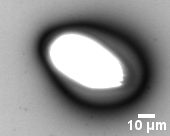
\includegraphics[width=4.0cm,height=4.0cm]{Figs/cuantificaciondefectos/hueco_cel_112.png}}{\caption{Defecto de superficie denominado hueco, de (48.45 $\pm$0.59)$\mu$m de diámetro equivalente. }\label{fig:huecocel}}
		\ffigbox{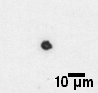
\includegraphics[width=4.0cm,height=4.0cm]{Figs/cuantificaciondefectos/mancha_cel_112.png}}{\caption{Defecto de superficie denominado mancha ó defecto de transmisión, de (6.33 $\pm$0.59)$\mu$m de diámetro equivalente.}\label{fig:manchacel}}
	\end{floatrow}
\end{figure}

Los defectos de superficie de un componente óptico pueden estar originados en el proceso de fabricación mismo, en el tratamiento y manipulación de la óptica (en inglés, \textit{handling}) en distintas etapas de un proceso de montaje ó en el transporte del proveedor al cliente. Estos defectos pueden provocar un cambio de las propiedades ópticas del componente, como por ejemplo una merma en la intensidad esperada ó una variación del espectro de tranmisión, y en consecuencia los usuarios finales de los componentes deben verificar la calidad óptica que los proveedores detallan en las especificaciones técnicas. A continuación se describen las dos especificaciones técnicas más utilizadas en la industria para determinar la calidad óptica de un componente, que son la \textit{U.S. Military Performance Specification} MIL-PRF-13830B y la ISO 10110 \cite{milprf}\cite{iso10110}.

\singlespacing
\subsection{MIL-PRF-13830B: especificaciones de \textit{scratch \& dig}}
\spacing{1.5}

\hspace{0.5cm}La especificación técnica MIL-PRF-13830B define los defectos permitidos en una superficie óptica utilizando una métrica dada por un par de números denominados \textit{scratch and dig numbers}: S/D. El \textit{scratch number} puede tomar alguno de los siguientes valores arbitrarios: 10,20,40,60,80, que representan en orden creciente el nivel de brillo de la rayadura. Este número no proviene de una medición experimental exacta, sino que es el resultado de comparar el brillo de la rayadura del componente a analizar con muestras de rayaduras calibradas como las que se muestran esquemáticamente en la Figura \ref{fig:scratchanddig}, bajo ciertas condiciones de iluminación específicas. En consecuencia, la asignación de un cierto \textit{scratch number} a un componente es una inspección visual subjetiva, es decir que varía de inspector a inspector.


\begin{figure}[H]
	\centering
	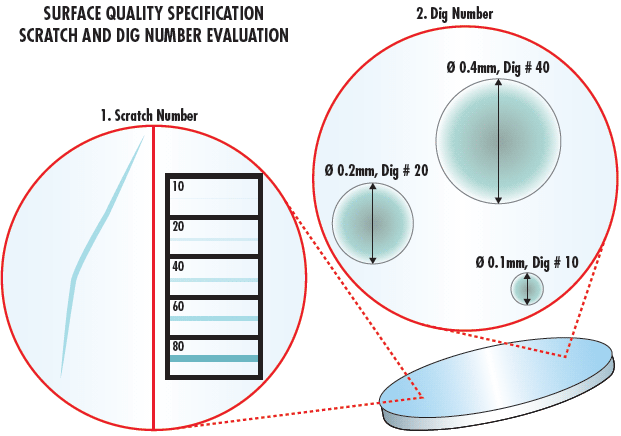
\includegraphics[scale=1.0]{Figs/cuantificaciondefectos/scratchanddig.png}
	\caption{El \textit{scratch number} es determinado a partir de la comparación de la rayadura de la óptica bajo análisis con las muestras calibradas, bajo ciertas condiciones de iluminación específicas. Adaptado de \href{https://bit.ly/2w1apWq}{\texttt{https://bit.ly/2w1apWq}}.}
	\label{fig:scratchanddig}
\end{figure}

Ahora bien, el \textit{dig number} es una cantidad medible experimentalmente: es el diámetro del hoyo más grande del componente, dado en $1/100$ de milímetros. Por ejemplo, un componente con un \textit{dig number} de 40 implica que el hoyo más grande de la óptica tiene un diámetro de 0.4 mm (Ver Figura \ref{fig:scratchanddig}). Luego de cuantificar todas las rayaduras y hoyos de la óptica, se determina el número de defectos permitidos de acuerdo a los siguientes criterios:
\begin{itemize}
\item La suma de todas las longitudes de las rayaduras con un cierto \textit{scratch number} (L$_{S_{\#}}$) no podrá superar el valor de un cuarto del diámetro ($\Phi$) de la óptica. Si el componente no tuviera una geometría circular, se considera el diámetro de un círculo con un área igual al de la óptica bajo análisis.
\begin{equation}
\sum L_{S_{\#}} < \frac{\Phi}{4}
\label{eq:snumb}
\end{equation}
\item El número total de hoyos de tamaño máximo permitido (N) no podrá exceder el diámetro de la óptica dividido por 20.
\begin{equation}
N  <  \frac{\Phi}{20}
\label{eq:nphi20}
\end{equation}
\item La suma de todos los diámetros (d) de los hoyos deberá ser menor ó igual al doble del número total de hoyos de tamaño máximo permitido (N) multiplicado por el \textit{dig number} (D$_{\#}$) especificado en fracciones de milímetros.
\begin{equation}
\sum d 	\leq 2 . N . D_{\#}
\label{eq:dmenorig}
\end{equation}
\end{itemize}

Así por ejemplo, una óptica de geometría circular con un diámetro de 200 mm y una calidad óptica especificada por el fabricante con \textit{scratch and dig numbers} S/D 30-20, puede tener rayones con un brillo calibrado de 30 y la suma de todas las longitudes de los rayones de brillo 30 no podrá ser superior a los 50 mm (de acuerdo a \eqref{eq:snumb}). Al mismo tiempo, la óptica no podrá tener más de 10 hoyos de tamaño máximo de 0.2 mm, es decir de \textit{dig number} igual a 20 (de acuerdo a  \eqref{eq:nphi20}) y la suma de los diámetros de todos los hoyos no podrá ser superior a los 4 mm (de acuerdo a \eqref{eq:dmenorig}).

La Figura \ref{fig:samplescratchs} muestra una comparación de cuatro muestras de calibración de rayaduras, medidas bajo idénticas condiciones de iluminación \cite{Aikens}.
\begin{figure}[H]
	\centering
	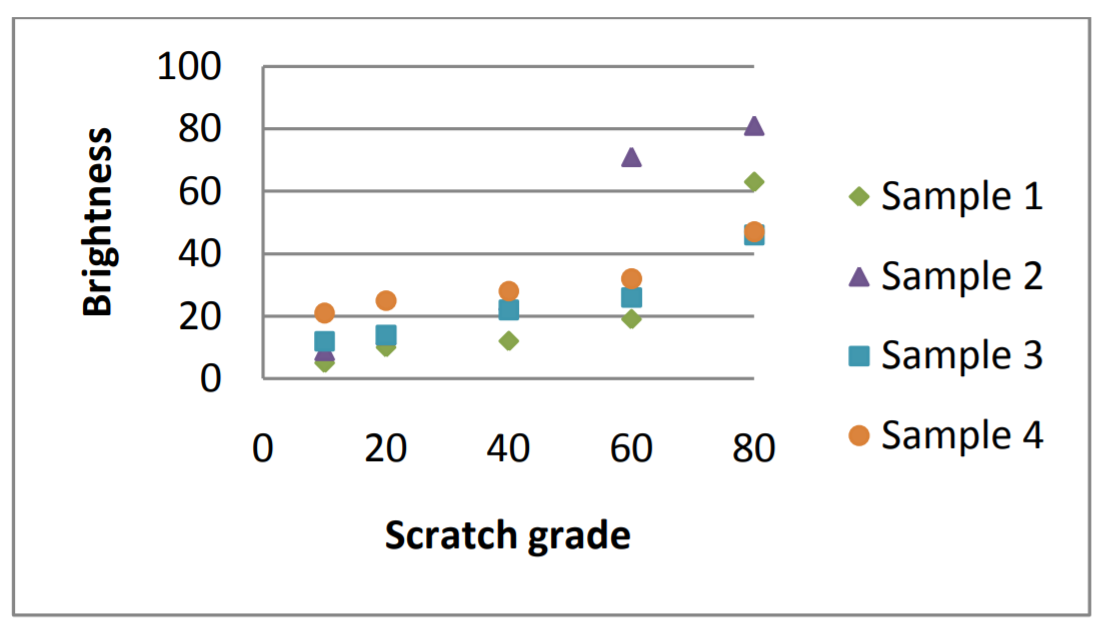
\includegraphics[scale=0.8]{Figs/cuantificaciondefectos/samplesscratch.png}
	\caption{Brillo relativo de cuatro muestras calibradas de \textit{scratch number}. \textit{Sample} en inglés significa muestra. La muestra 1 es de la empresa FLIR/Brysen (S\&D 1109), la muestra 2 es de Davidson Optronics (D-667A S/N 2431), la muestra 3 es de Eastman Kodak (\textit{paddle} EKCO CM2) y la muestra 4 es de Jenoptik (\textit{paddle} EO \#53-157 CM1). La muestra 4 es vendida comercialmente por los proveedores Edmund Optics y por Thorlabs. Gráfico tomado de \cite{Aikens}.}
	\label{fig:samplescratchs}
\end{figure}


De la Figura \ref{fig:samplescratchs} se desprende que las cuatro muestras son incompatibles entre sí, es decir arrojan resultados de brillo distintos entre sí para un cierto \textit{scratch number}. Se observa que para un \textit{scratch number} igual a 10, el brillo de la muestra 4 es más brillante que el \textit{scratch number} 60 de la muestra 1.
Así también el brillo del \textit{scratch number} 60 de la muestra 2 es más de dos veces más brillante que cualquiera de las otras muestras para este mismo \textit{scratch number}. 

Si bien la métrica de \textit{scratch and dig} sigue siendo ampliamente utilizada en la industria, el hecho de que el análisis de las rayaduras sea dependiente del inspector de turno sumado a que las muestras de brillo calibradas varían de acuerdo al fabricante de las mismas, hacen que estas especificaciones técnicas para determinar la calidad de una óptica resulten técnicamente ambiguas. A continuación se explican las especificaciones técnicas de la ISO 10110 y se hace notar que ambas especificaciones técnicas figuran en la hoja de datos del filtro analizado en el presente trabajo. Luego se muestran las características del filtro analizado en esta tesis junto a sus especificaciones ópticas.

\singlespacing
\subsection{ISO 10110: defectos de superficie}
\spacing{1.5}


\hspace{0.5cm}Las especificaciones de la ISO 10110 determinan de forma cuantitativa el tamaño y número de defectos de superficie que un componente óptico puede presentar. El concepto de defecto de superficie para esta normativa se corresponde con la definición de defecto dada en la primera sección de este capítulo (Ver \hyperref[sec:defectsurf]{def.}). Es decir, contiene a todos los tipos de defectos que representan una inhomogeneidad en la superficie óptica del componente. Esto es, no distingue las rayaduras de los hoyos ni de cualquier otro tipo de defecto para determinar la calidad óptica de un componente.

La normativa ISO 10110 indica el número de defectos permitidos ($N_{p}$) y un coeficiente dado en fracciones de milímetros denominado \textit{grade number} ($A_{g}$) que es igual a la raíz cuadrada del área del defecto de tamaño máximo permitido. Estos dos valores son expresados en las hojas de datos de los componentes ópticos de la siguiente manera: 5/$N_{p}$x$A_{g}$. El número 5 hace referencia a que la especificación técnica dada se refiere a las tolerancias de los defectos de superficie. A su vez, el área del componente óptico cubierta por los defectos permitida está dada por la siguiente expresión:

\begin{equation}
A_{defectos} = N_{p}\hspace{2pt} .\hspace{2pt} A_{g}^{2}
\end{equation}

Por ejemplo, la especificación 5/5x0.05 brindada por un cierto fabricante, indica que el componente cumple que tiene como máximo 5 defectos de 50 micrones y el área máxima cubierta por los defectos puede ser de 12500 $\mu m^{2}$.

Se hace notar que el control de calidad de los componentes ópticos bajo la normativa ISO 10110, al ser meramente cuantitativo, resulta más preciso y objetivo que el control de calidad bajo las especificaciones de \textit{scratch \& dig}. Mientras que para esta última normativa, el control de calidad del componente suele ser realizado por un técnico entrenado vía una inspección visual, para el análisis de las especificaciones de la ISO 10110 de un cierto componente, se utilizan microscopios con la suficiente magnificación como para poder cuantificar los defectos.

%\begin{tcolorbox}[colback=blue!10!white,colframe=blue!43!black]
 En esta sección se definió el concepto de defecto de superficie de un componente óptico como cualquier inhomogeneidad presente en la superficie bajo análisis. Se describieron las dos especificaciones técnicas más utilizadas para determinar la calidad óptica de la superficie de un componente, ambas presentes en la hoja de datos del filtro a analizar en la presente tesis. Por un lado, las especificaciones de \textit{scratch \& dig} que resultan un poco ambiguas debido a la determinación subjetiva de los \textit{scratch numbers} del componente. Y, por otro lado, la ISO 10110 que propone superar esta ambiguedad no distinguiendo los tipos de defectos presentes en la óptica, sino tratándolos a todos por defectos en general por igual. Ahora bien, en la práctica, la mayoría de los proveedores (entre ellos Edmund Optics, Thorlabs) en la actualidad utilizan las especificaciones de \textit{scratch \& dig} para indicar la calidad de la superficie óptica del componente en cuestión. 
 
 A continuación se describen las características y dimensiones del filtro analizado en este trabajo y luego se describe el análisis de la cuantificación de los defectos determinados en el filtro a partir de la adquisición de imágenes por transmisión con un microscopio.

\singlespacing
\section{Características del filtro}
\spacing{1.5}

\hspace{0.5cm}El componente óptico analizado en la presente tesis, denominado en adelante simplemente filtro, consiste de un arreglo de cinco filtros ópticos de interferencia  considerados en adelante a cada uno de ellos como una banda. En la Figura \ref{fig:filtroposta} se muestra el filtro real analizado y en la Figura \ref{fig:dimsfiltr} se muestran las diimensiones especificadas por el fabricante.

Las zonas (en inglés, \textit{zone}) están asociadas a una cierta banda espectral de transmisión de la siguiente manera:
\begin{itemize}
\item Zona 1 - Banda Azul: (450-510) nm
\item Zona 2 - Banda Verde: (510-580) nm
\item Zona 3 - Banda Pancromática\footnote{La palabra pancromática, del griego ático donde pan significa todo y cromático viene de la familia de la palabra color, implica que dicha banda tiene un espectro de transmisión en toda la región del visible.}: (450-750) nm
\item Zona 4 - Banda Roja: (590-690) nm
\item Zona 5 - Banda NIR\footnote{NIR, en inglés \textit{Near-Infrared}, se le denomina a la región espectral del infrarrojo cercano que se extiende aproximadamente desde los 780 nm hasta los 2000 nm.}: (750-900) nm
\end{itemize}
 


\begin{figure}[H]
	\begin{floatrow}
		\ffigbox{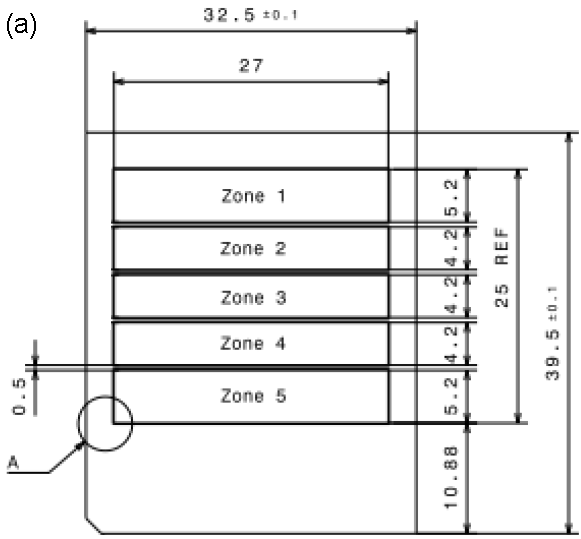
\includegraphics[scale=0.8]{Figs/cuantificaciondefectos/dimsfiltro.png}}{\caption{Dimensiones del filtro especificadas por el fabricante.}\label{fig:dimsfiltr}}
		\ffigbox{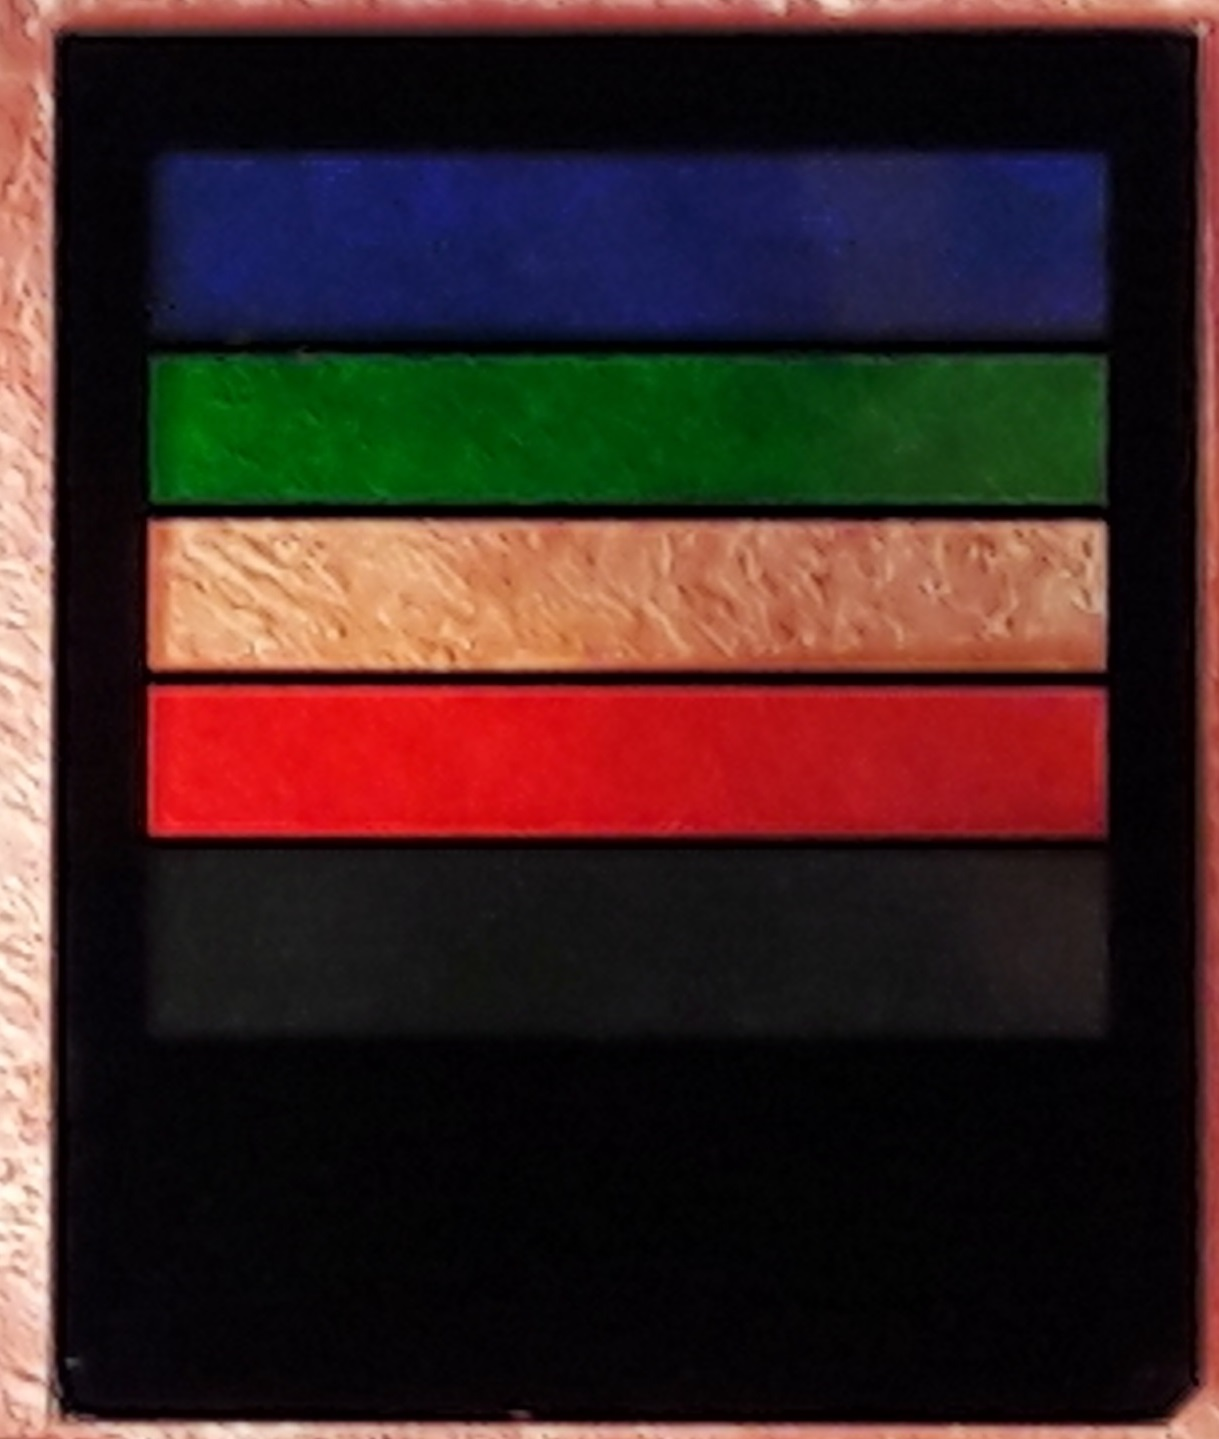
\includegraphics[scale=0.15]{Figs/cuantificaciondefectos/filtro_real.jpg}}{\caption{Imagen del filtro real analizado.}\label{fig:filtroposta}}
	\end{floatrow}
\end{figure}

Las especificaciones ópticas de la calidad de la superficie del filtro brindadas por el fabricante son las siguientes:
\begin{center}
5/2x0.063 (\textit{according to MIL PRF 13830, S/D 20-10}).
\end{center}

Estas especificaciones implican para el caso de la ISO 10110, 5/2x0.063, que en la superficie óptica del filtro puede haber un máximo de 2 defectos de 63 micrones de lado y que el área total máxima cubierta por defectos puede ser de 7938 $\mu m^{2}$. Y, las especificaciones de \textit{scratch \& dig}, S/D 20-10, indican que puede haber rayaduras con un brillo calibrado de 20 (de acuerdo a una muestra calibrada indicada por el proveedor) y que la suma de todas las longitudes de las rayaduras de brillo 20 no podrá ser superior a los 7.5 mm (de acuerdo a \ref{eq:snumb})\footnote{ El diámetro equivalente del filtro es de $(30.0 \pm 0.1 )mm$, si se considera el área útil del filtro como la región central que comprende a las bandas que es de $((25.0 \pm 0.1)mm$ x $(27.0 \pm 0.1) mm = (675 \pm 4) mm^{2}$}. El filtro no deberá tener más de 2 hoyos de tamaño máximo de 100 $\mu m$  (de acuerdo a \ref{eq:nphi20}) y la suma de los diámetros de todos los hoyos no podrá ser superior a los 0.4 mm (de acuerdo a \ref{eq:dmenorig}).

Se hace notar que entre las bandas se encuentran unas banditas de un material no declarado por el fabricante, denominado en adelante cromo, de $(0.5 \pm 0.1)mm $ de largo como se muestra en la Figura \ref{fig:dimsfiltr}. El mismo material cubre toda la región del filtro no contenida por las cinco bandas.

A continuación se describe el proceso de adquisición de las imágenes del filtro, posteriormente su procesamiento y el algoritmo de detección de los defectos y por último se discute un análisis cuantitativo de los mismos.



\singlespacing
\section{Adquisición de las imágenes del filtro}
\label{sec:conf}
\spacing{1.5}


\hspace{0.5cm}Para la adquisición de las imágenes del filtro se utilizó un microscopio invertido Zeiss Axio Observer Z1 como se muestra en la Figura \ref{fig:ZEISSdellabo}, con un objetivo Zeiss N-Achroplan de magnificación 10X y apertura numérica de 0.25.
\begin{figure}[H]
	\centering
	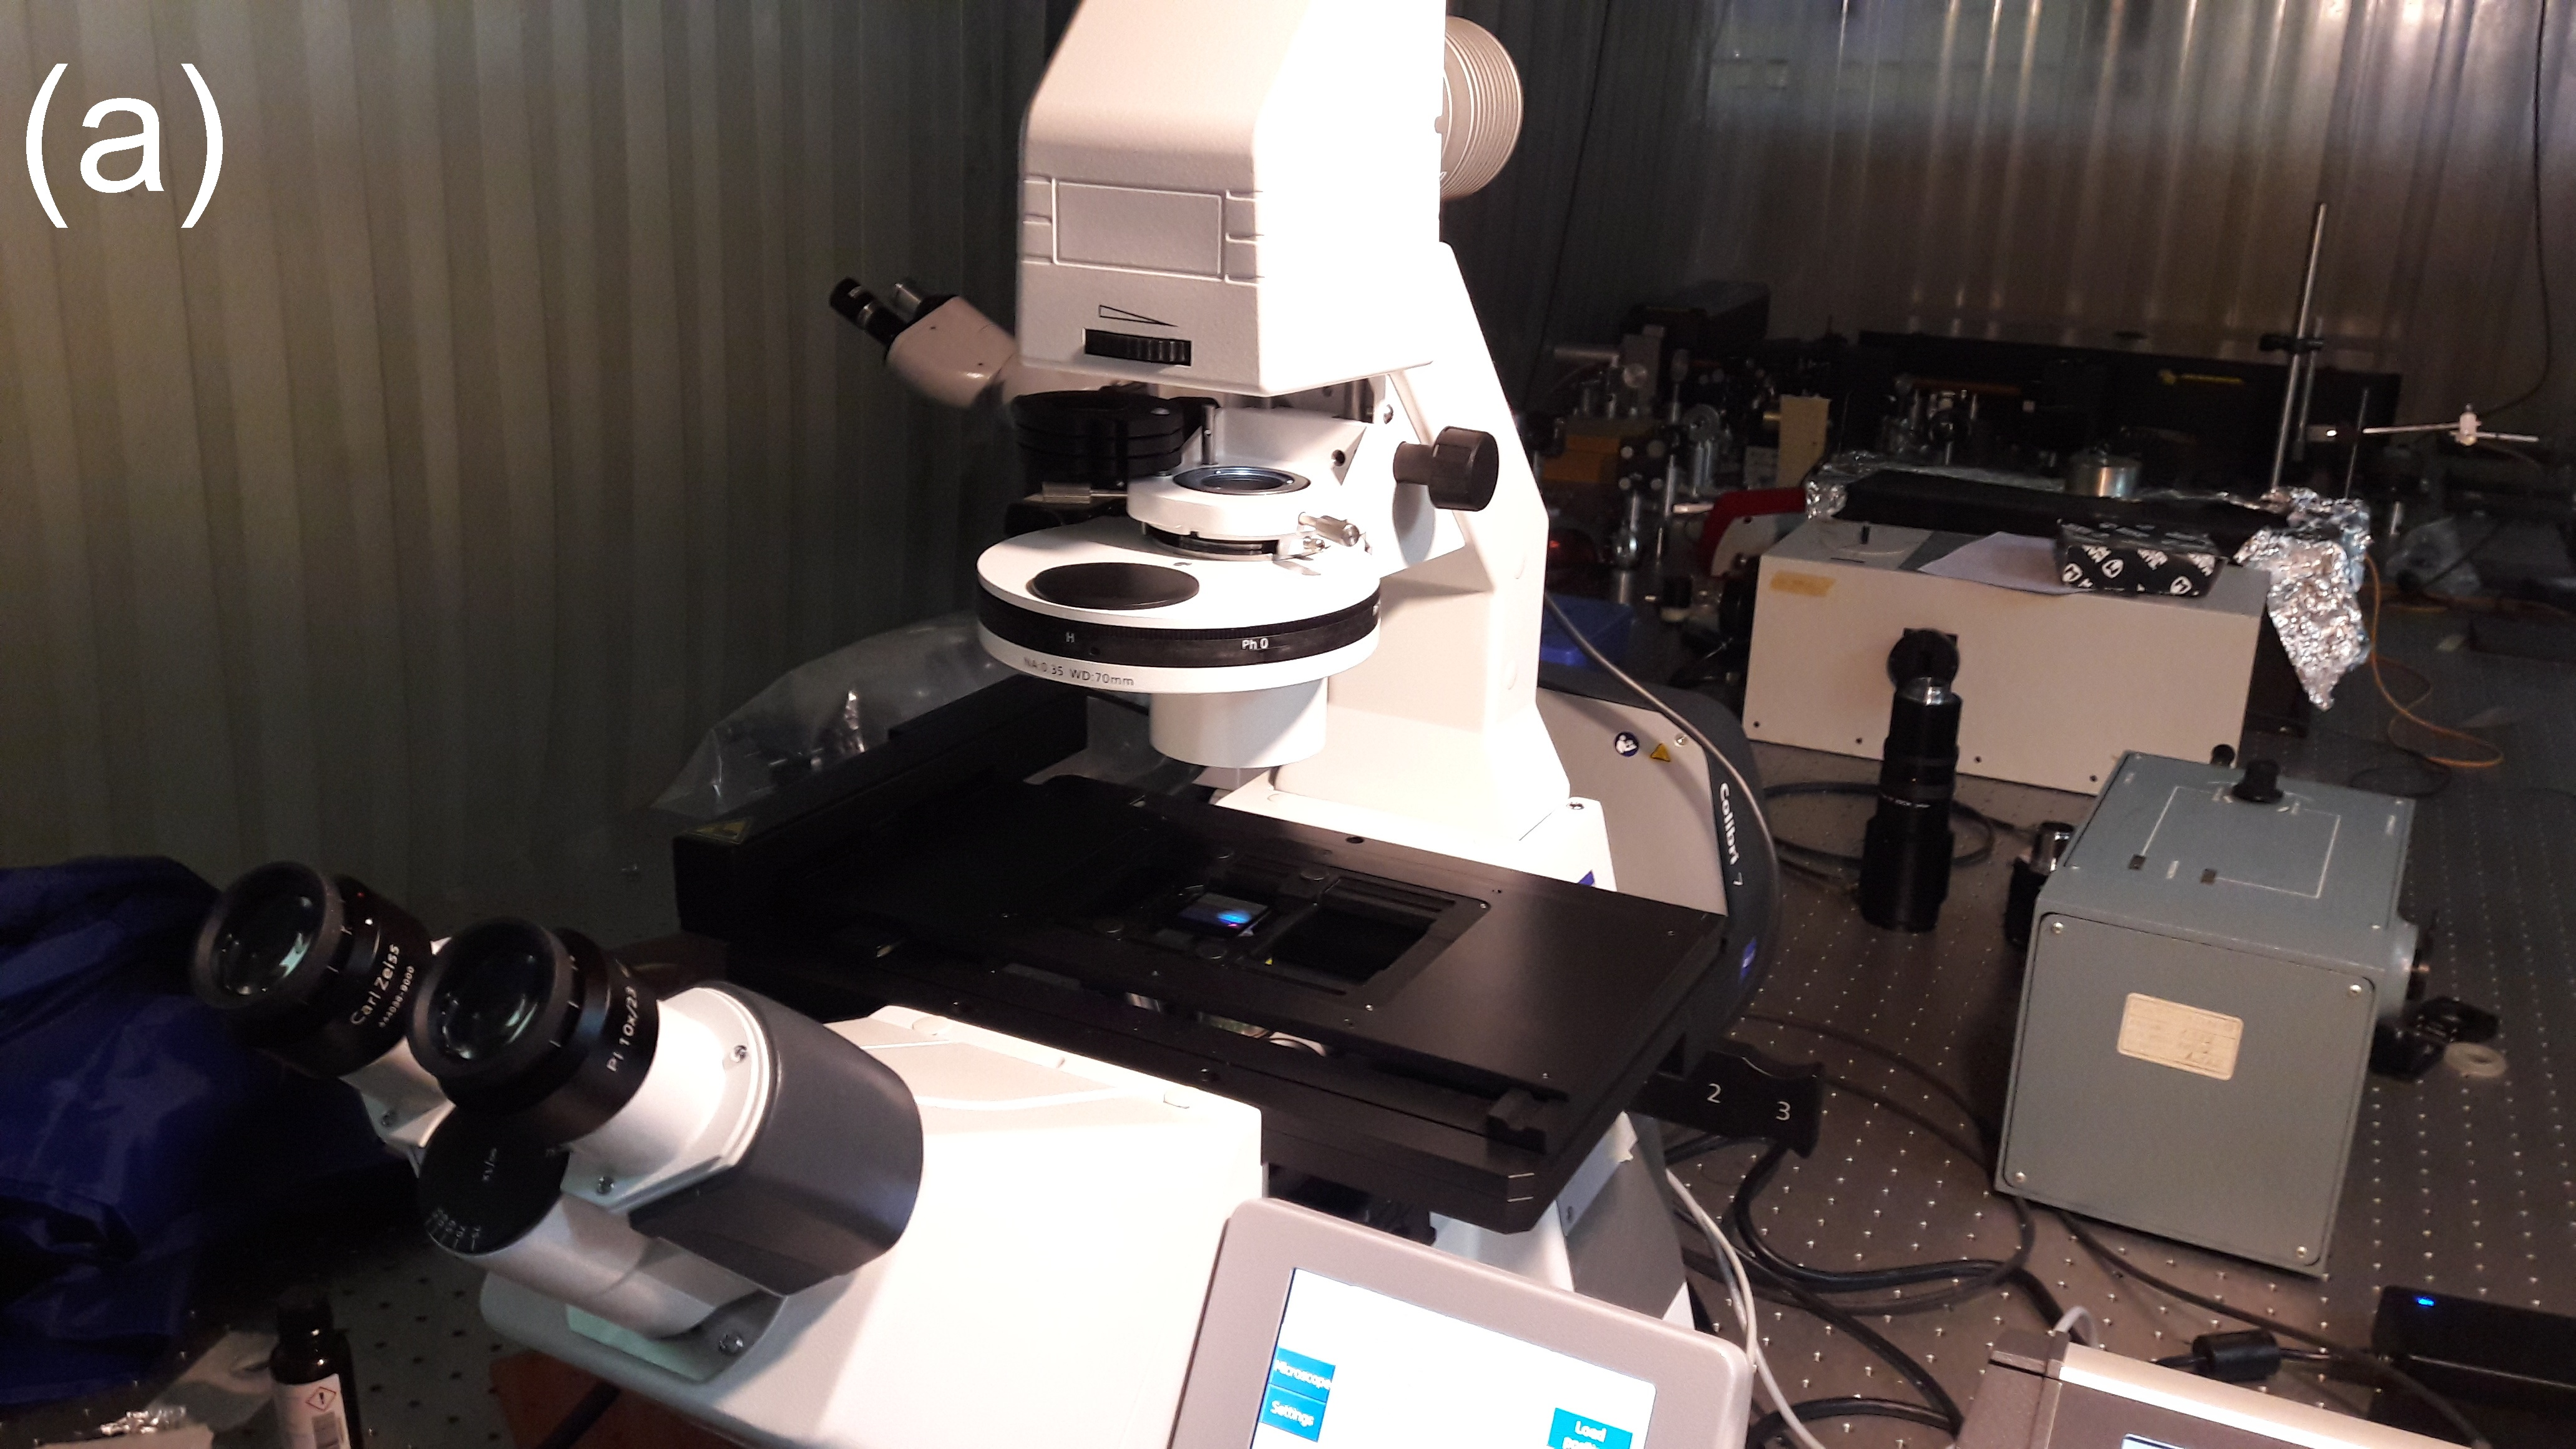
\includegraphics[scale=0.08]{Figs/defectosZEISS/b.jpg}
	\caption{Microscopio invertido Zeiss Axio Observer Z1.}
	\label{fig:ZEISSdellabo}
\end{figure}

Las imágenes del filtro fueron adquiridas por transmisión utilizando una fuente de luz blanca, en condiciones de \textit{bright field}\footnote{Técnica de iluminación que en castellano suele ser denominada de 'campo brillante' para diferenciarla de la iluminación de campo oscuro (en inglés \textit{dark field}).}. Se montó el filtro sobre el portamuestras de la platina del microscopio como se muestra en la Figura \ref{fig:filtroenZEISS} y mirando por el ocular se puso en foco la superficie del filtro a medir.  
\begin{figure}[H]
	\centering
	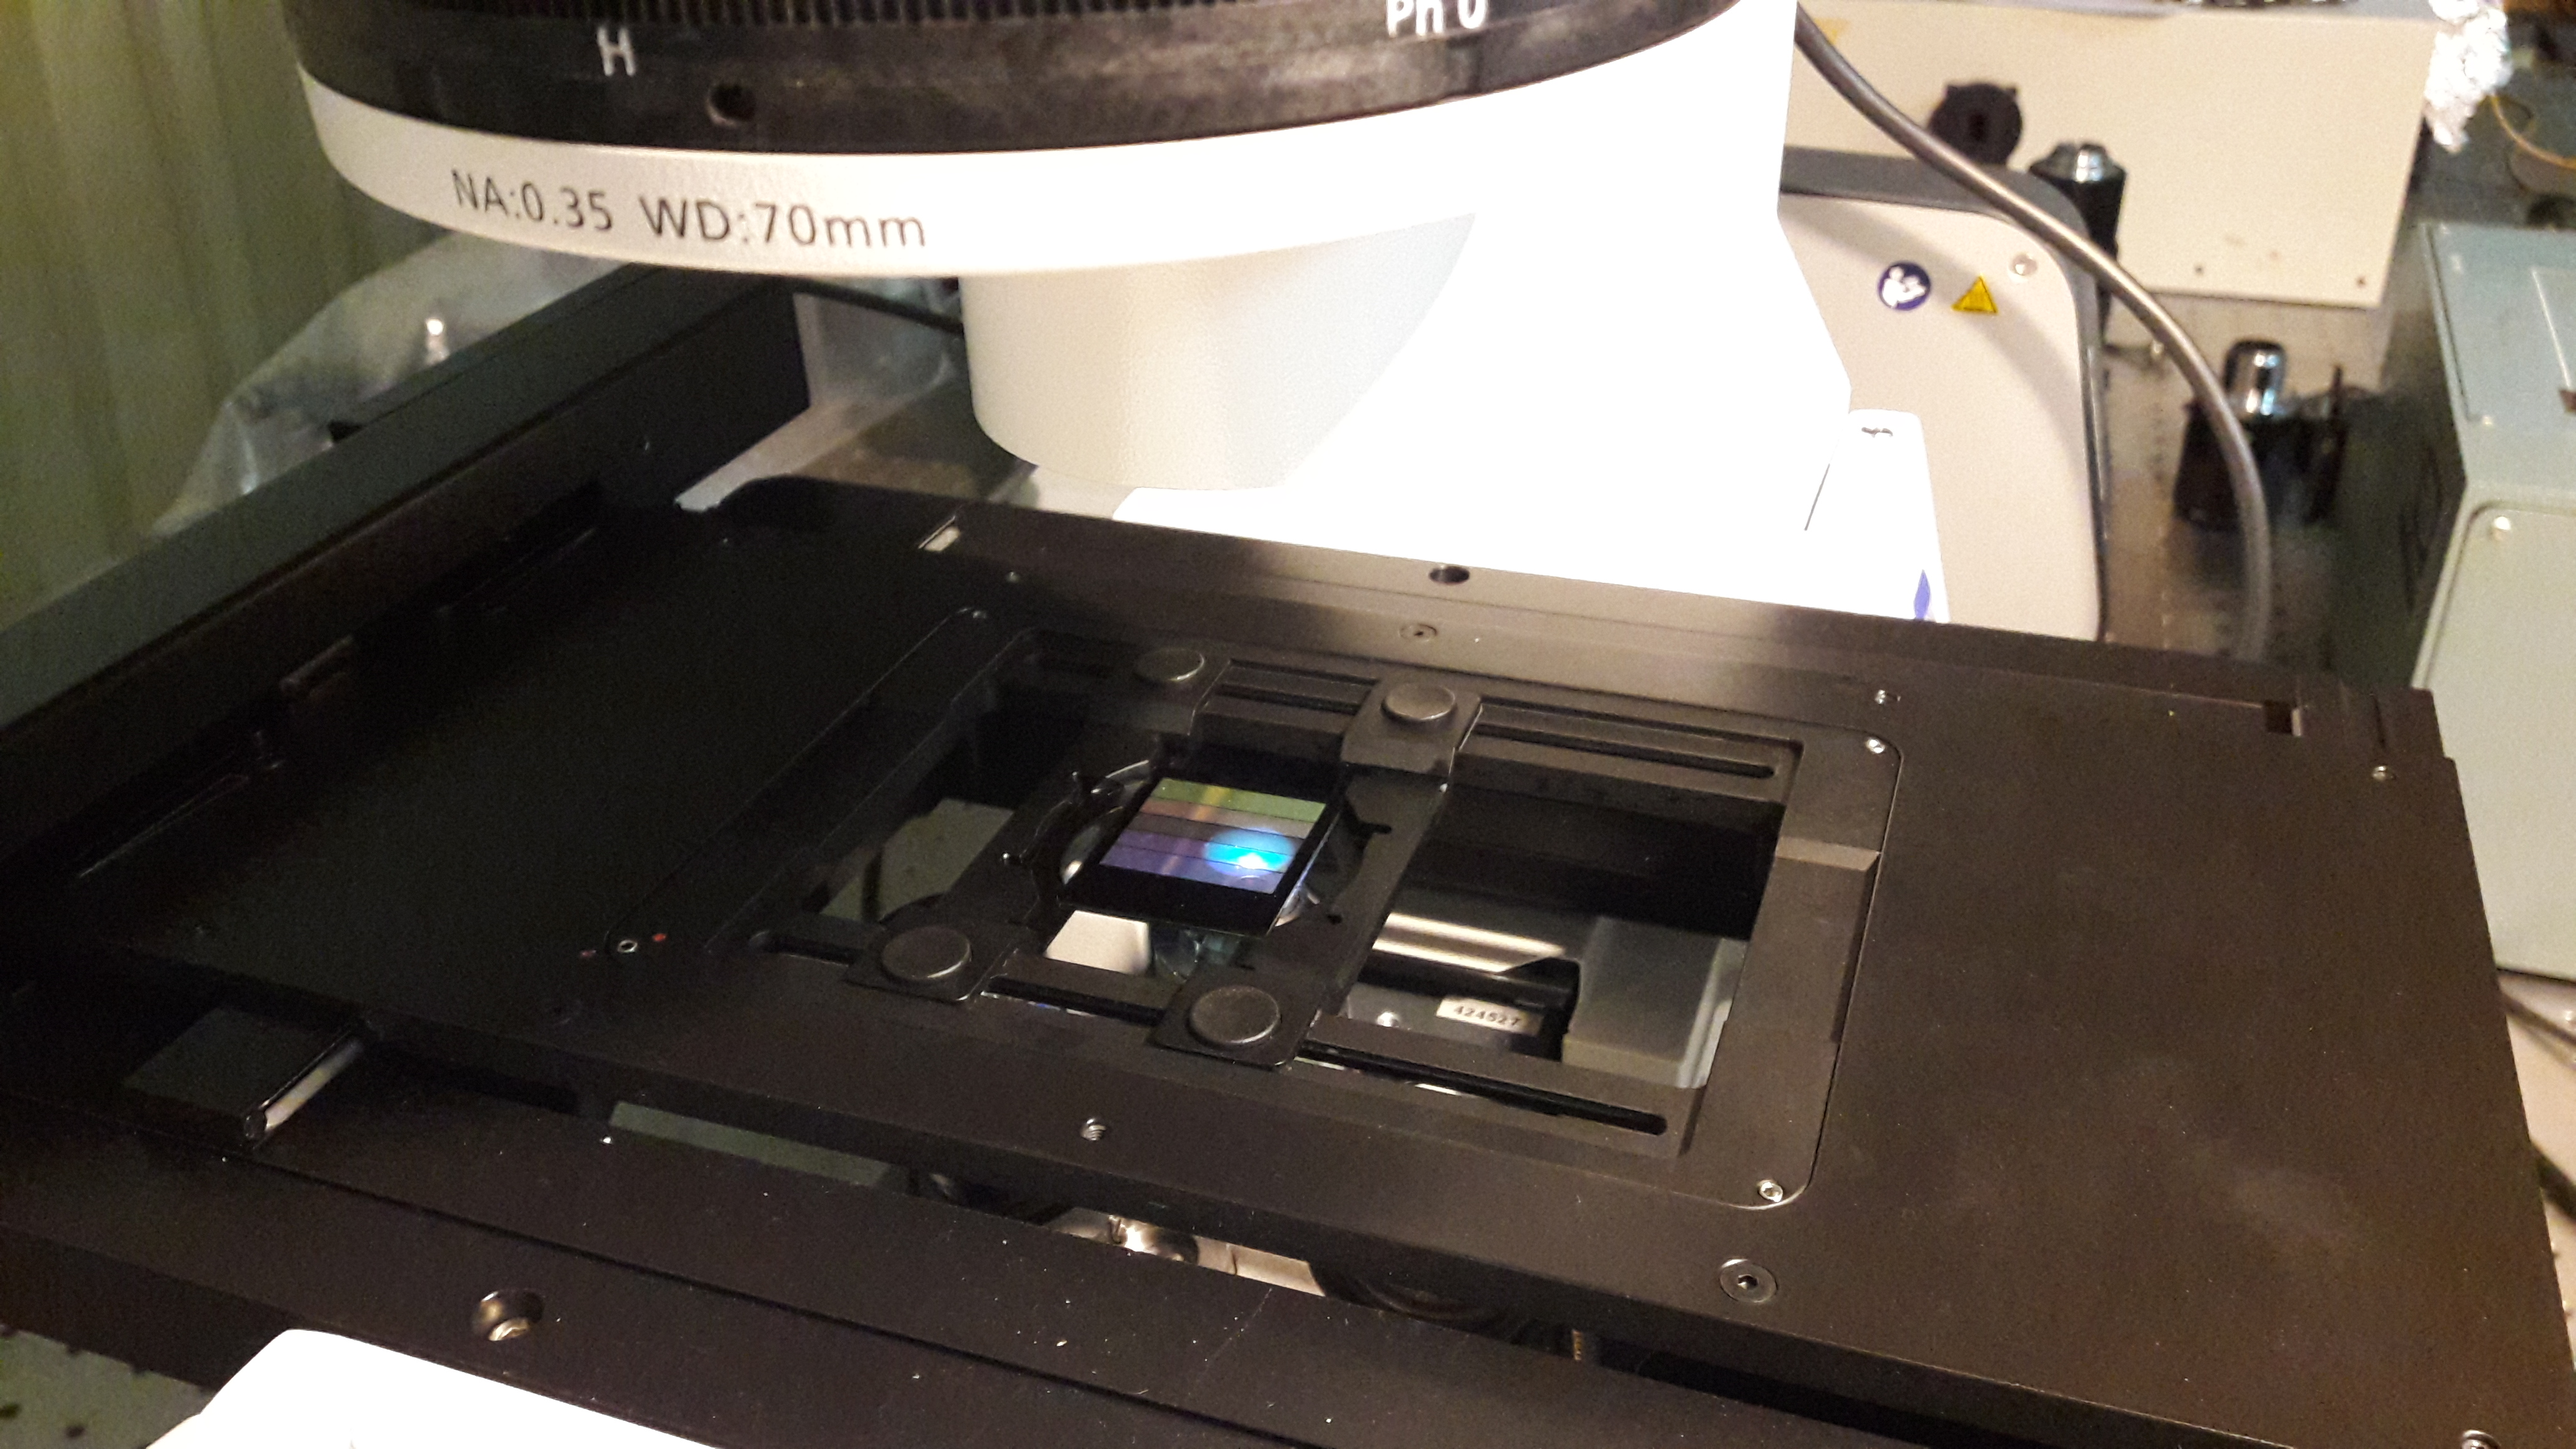
\includegraphics[scale=0.08]{Figs/defectosZEISS/a.jpg}
	\caption{Montaje del filtro sobre el portamuestras de la platina del microscopio.}
	\label{fig:filtroenZEISS}
\end{figure}
La cámara monocromática del microscopio del fabricante Zeiss, modelo Axiocam 702, con un sensor CMOS de 1/1.2'' (diagonal de 13.3mm) y una resolución de 2.3 megapíxeles (1216x1920 píxeles), fue controlada a través del software ZEN 2.5 (\textit{Blue edition}, 2018) del mismo fabricante. Se utilizó la calibración de la cámara que viene de fábrica del microscopio para la configuración utilizada (Ver \hyperref[sec:conf]{config.}), donde las medidas de 1 píxel son de 0.586 $\mu m$ x 0.586 $\mu m$. Cada \textit{tile} individual tiene dimensiones de 713 $\mu m$ x 1125 $\mu m$. 

Se configuró el software para adquirir las imágenes por transmisión, en particular se eligió la fuente de luz blanca y para cada medición su intensidad, además del tiempo de exposición de la cámara. Como la cámara tiene otro arreglo óptico que el ocular, el plano focal de la superficie del filtro elegida para medir se encuentra a una distancia distinta entre el objetivo y la muestra. En consecuencia, con las perillas manuales del microscopio se pone en foco la imagen observando la adquisición en vivo en la computadora. 


\singlespacing
\subsection{\textit{Tile scan}}
\spacing{1.5}

\hspace{0.5cm}A continuación se explica cómo se adquirieron las imágenes para una determinada región del filtro, ya sea para el filtro completo a excepción de la banda del NIR ó para cada banda espectral del filtro en particular.

La palabra en inglés \textit{tile} significa baldosa(ver Figura \ref{fig:tilescan}) en castellano y realizar un \textit{tile scan} implica realizar un barrido de adquisición de imágenes de una cierta área a elección de una muestra donde el área total a adquirir está compuesta por múltiples baldosas. Cada baldosa, es decir cada \textit{tile} constituye una imagen del microscopio de acuerdo al \textit{field of view} (FOV) \footnote{En castellano es el campo de visión y representa el área física de la imagen, que para el caso de una cámara el FOV viene dado por el cociente entre el tamaño del sensor CMOS y la magnificación del microscopio.} que se tiene del arreglo óptico de la cámara integrada al microscopio.

Hay distintas formas de elegir el área total a adquirir en el software. Se eligió la opción de determinar la región a adquirir a partir de la selección visual individual de las cuatro esquinas de la misma, como se muestra en la Figura \ref{fig:tilescan}. Para elegir estas esquinas el microscopio cuenta con un \textit{joystick} que permite mover la platina motorizada del microscopio en el plano de la imagen.

\begin{figure}[H]
	\centering
	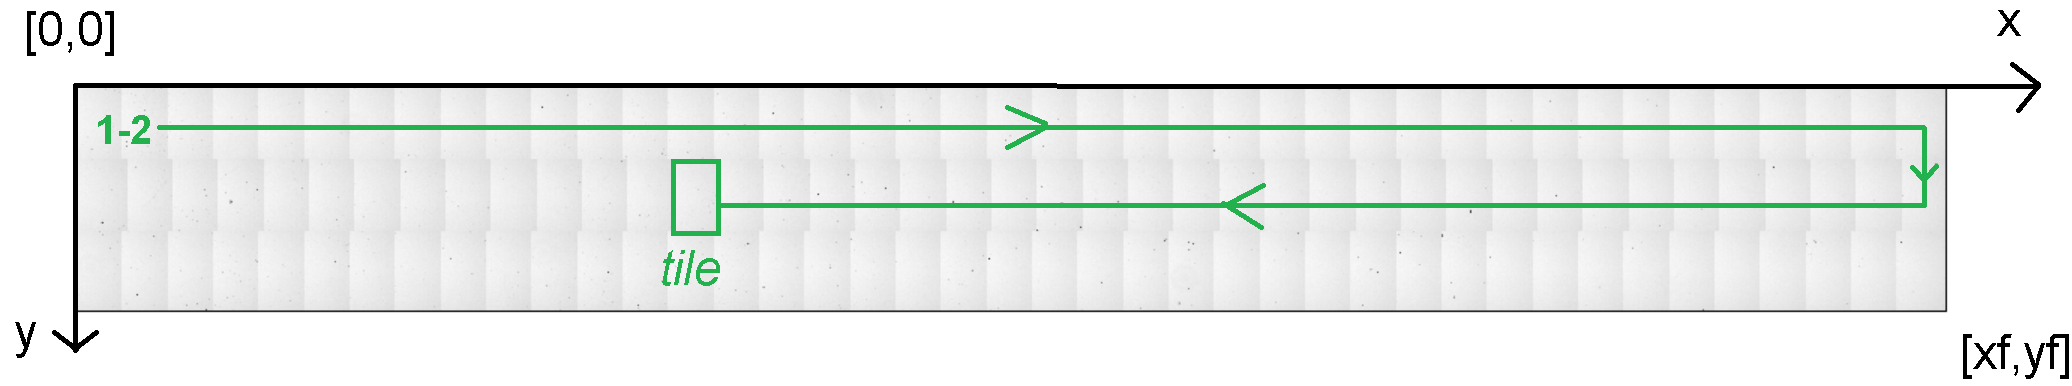
\includegraphics[width=1.0\textwidth]{Figs/cuantificaciondefectos/tilescan.png}
	\caption{\textit{Tile scan} de la banda pancromática.}
	\label{fig:tilescan}
\end{figure} 

Entre otros parámetros del barrido, se elige el \textit{overlap} entre las baldosas, es decir la superposición entre las mismas que luego permite obtener una imagen completa individual para su visualización,  realizando un \textit{stitching}\footnote{El \textit{stitching} es el proceso computacional por el cual se combinan múltiples \textit{tiles} para
producir una sola imagen que permita una mejor visualización (Ver técnica SIFT (\textit{Scale Invariant Feature Transform}), \cite{Lowe}).} como post-procesamiento de las imágenes. Este último procedimiento también fue realizado con el software de Zeiss. Se configuró el \textit{overlap} en 10$\%$ para todas las mediciones, siendo este valor el mínimo encontrado para que el \textit{stitching} entre las imágenes consecutivas sea realizado correctamente sin dejar espacios en blanco y para que dicha superposición elimine de la imagen la menor cantidad de defectos posibles. Por último, se elige en la configuración que cada baldosa sea exportada como una imagen individual para su posterior análisis.

\begin{warningbox}{}
\faExclamationTriangle \hspace{2pt} \texttt{Advertencias:}\par
\begin{itemize}
\justifying
\item Cada barrido completo de una banda es guardado por el software de Zeiss en un archivo de extensión .czi que contiene toda la \textit{metadata} como la información referida a la configuración del microscopio utilizada. Dicho archivo puede ser manipulado con el software de Zeiss, ó con el \href{https://imagej.net/Fiji}{Fiji-ImageJ} (tiene más herramientas que el software ImageJ a secas) ó a través del lenguaje \textit{python} utilizando la librería \href{https://pypi.org/project/czifile/}{\textit{czifile}} (Ejemplo sencillo: \href{https://github.com/jrr1984/defects_analysis/blob/master/zeiss_cfi.ipynb}{\faGithub}).
\item El archivo .czi de la banda completa además contiene todas las \textit{tiles} del barrido que pueden ser exportadas como archivos individuales utilizando las herramientas de procesamiento del software de Zeiss \cite{tilezeiss}. Es muy importante exportar dichas imágenes eligiendo un formato de imagen que no modifique la calidad de la imagen original, esto es, que no se pierda precisión sobre los valores de intensidad de cada píxel. 
\item Se recomienda para el guardado, manipulación, operaciones, etc., utilizar el formato de imagen TIFF (\textit{Tagged Image File Format}) pues es un formato que guarda los datos de intensidad de cada píxel originales, sin pérdida de precisión por compresión. Y, definitivamente no se puede utilizar el formato de imagen JPEG (\textit{Joint Photographic Experts Group}) en el campo de la microscopía pues el tipo de compresión que realiza sobre los datos originales resulta en una pérdida de precisión.
\item Por último, se hace notar que la pérdida de precisión de una imagen puede ocurrir tanto en el guardado como en las operaciones sobre las imágenes. Un ejemplo de esta pérdida de precisión sería convertir las imágenes de una precisión original de 16 bits ($2^{16} = 65536$ posibles valores de intensidad) a una precisión de 8 bits ($2^{8} = 256$). Este inconveniente podría ser producido automáticamente por ejemplo en alguna operación utilizando la librería \textit{scikit-image} \cite{van2014scikit}, por lo que se sugiere controlar la precisión con la que se manipulan las imágenes en cada operación realizada.
\end{itemize}

\end{warningbox}	

\singlespacing
\subsection{Superficies y mapa de los defectos del filtro}
\spacing{1.5}

\hspace{0.5cm}Se adquirieron imágenes completas del filtro, a excepción de la banda espectral del NIR, para las dos superficies exteriores del filtro como se muestra en las Figuras \ref{fig:supfiltrocondensador} y \ref{fig:supfiltroobjetivo}. Las dos superficies exteriores denominadas arbitrariamente A y B son las que se muestran especificadas en la Figura \ref{fig:espfil} y que se encuentran en la interfaz filtro-aire.

\begin{figure}[H]
	\begin{floatrow}
		\ffigbox{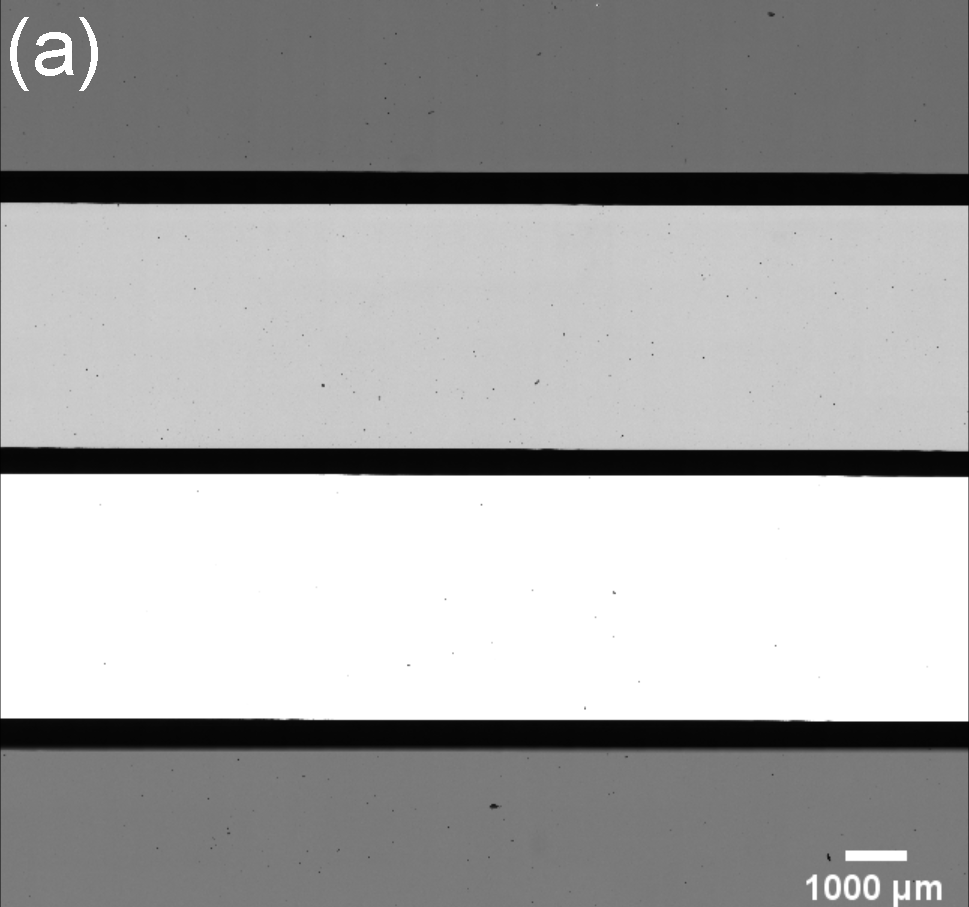
\includegraphics[width=7.25cm,height=9.0cm]{Figs/cuantificaciondefectos/supextex2216.png}}{\caption{Imagen de la superficie exterior A del filtro, para un barrido de 15.54 mm x 14.94 m.}\label{fig:supfiltrocondensador}}
		\ffigbox{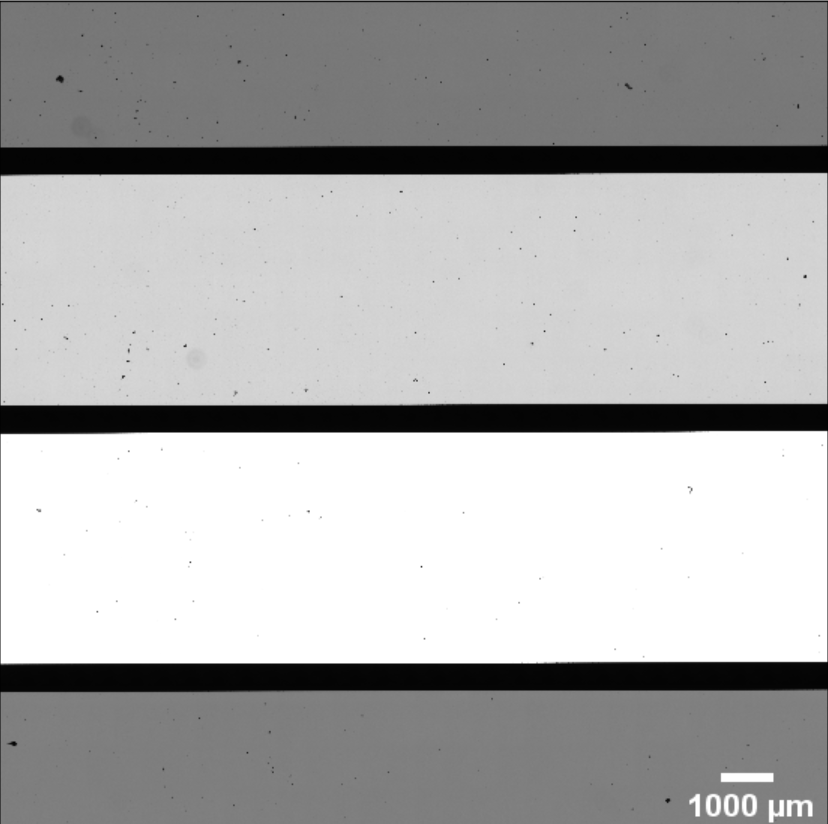
\includegraphics[width=7.25cm,height=9.0cm]{Figs/cuantificaciondefectos/supextex1515.png}}{\caption{Imagen de la superficie exterior B del filtro, para un barrido de 15.50 mm x 15.55 mm.}\label{fig:supfiltroobjetivo}}
	\end{floatrow}
\end{figure}

\begin{figure}[H]
	\centering
	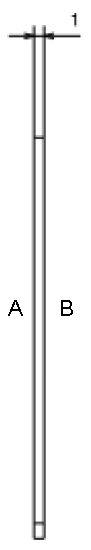
\includegraphics[scale=0.5]{Figs/cuantificaciondefectos/espesorfiltro.png}
	\caption{Dimensiones del espesor del filtro. Las superficies exteriores del filtro son las superficies A y B, que se encuentran en la interfaz filtro-aire.}
	\label{fig:espfil}
\end{figure}

En las Figuras \ref{fig:supfiltrocondensador} y \ref{fig:supfiltroobjetivo} se muestran las bandas espectrales del filtro en orden descendente: Azul (450-510 nm), Verde (510-580 nm), Pancromática (450-750 nm), Roja (590-690 nm). El brillo, el contraste y el tamaño de las imágenes originales fueron modificados para obtener una mejor visualización, utilizando el software FIJI-ImageJ. 

Para realizar el barrido completo de cada superficie se verificó en las cuatro esquinas de la superficie a medir que no se pierda el foco de la imagen. Se eligió la intensidad de la fuente de luz y el tiempo de integración de la cámara tales que no saturen alguna de las bandas del filtro de forma tal poder adquirir una imagen completa del filtro en un solo barrido, y de forma tal que se utilice la mayor parte del rango dinámico de la cámara, como se puede ver en el histograma de la intensidad de los píxeles de la Figura \ref{fig:histograma15x15} para el barrido de la superficie A del filtro.

\begin{figure}[H]
	\centering
	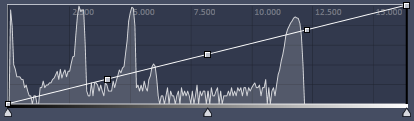
\includegraphics[width=1.0\textwidth]{Figs/defectosZEISS/histograma15x15.png}
	\caption{Histograma de la intensidad de los píxeles de la cámara del barrido de la superficie exterior A del filtro.}
	\label{fig:histograma15x15}
\end{figure}

Se hace notar que la banda del NIR no pudo ser adquirida en el barrido completo de las superficies exteriores del filtro pues con los valores de intensidad de la lámpara y del tiempo de adquisición de la cámara fijados para que ninguna de las bandas del filtro sature, no era posible obtener una imagen de esa banda. Si bien la cámara tiene un rango de sensibilidad espectral comprendido entre los 350 nm y los 1000 nm de acuerdo a su hoja de datos \cite{Zeiss}, del gráfico de la eficiencia cuántica\footnote{La eficiencia cuántica, en inglés \textit{Quantum efficiency} (QE), es una medida precisa de la sensibilidad de un dispositivo fotosensible que permite determinar como es la respuesta del dispositivo para cada longitud de onda.} se desprende que para la región espectral del NIR tiene una eficiencia cuántica menor al 30\% (Ver Figura \ref{fig:eficienciacuanticamara}). A esto se le suma el hecho de que la fuente de luz tiene un espectro de emisión de baja intensidad en la región del NIR, como se muestra en el gráfico de la intensidad en función de la longitud de onda de la Figura \ref{fig:espectrolamparazeiss}. Dicho espectro fue medido con el espectrómetro CCS200 de Thorlabs. 


\begin{figure}[H]
	\centering
	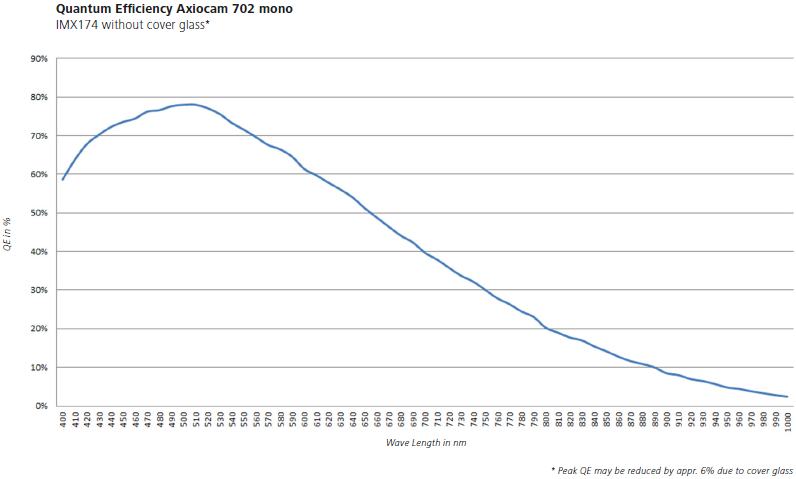
\includegraphics[width=1.0\textwidth]{Figs/defectosZEISS/eficienciacuanticacamarazeiss.png}
	\caption{Gráfico de la eficiencia cuántica de la cámara monocromática del microscopio Aiocam 702 en función de la longitud de onda.}
	\label{fig:eficienciacuanticamara}
\end{figure}



\begin{figure}[H]
	\centering
	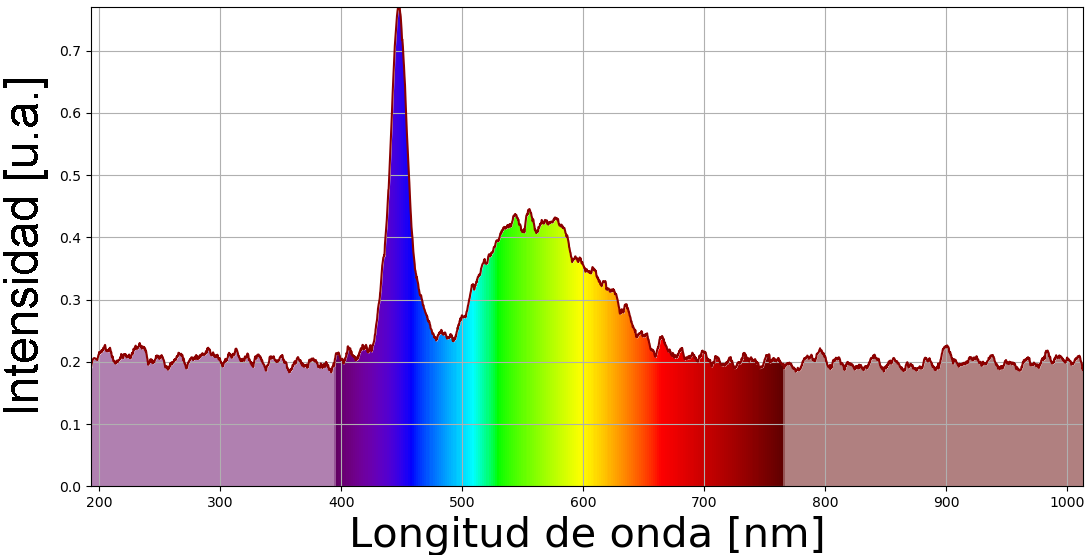
\includegraphics[width=1.0\textwidth]{Figs/defectosZEISS/espectrolampZEISSacolor.png}
	\caption{Espectro de emisión de la fuente de luz del microscopio.}
	\label{fig:espectrolamparazeiss}
\end{figure}

Ahora bien, la banda espectral del NIR fue medida individualmente posteriormente como se explica más adelante. Para poder obtener una imagen del filtro completo, incluida la banda del NIR, se debería cambiar la fuente de luz por una que tenga una mayor intensidad en dicha región espectral.

La imagen completa de cada superficie exterior del filtro permitió:
\begin{itemize}
	\item Realizar un primer diagnóstico visual por imagen de la calidad óptica de construcción del filtro. 
	\item Determinar que ninguna de las dos superficies exteriores del filtro presentaba una cantidad mayor notable de defectos que la otra como se puede observar en las Figuras \ref{fig:supfiltrocondensador} y \ref{fig:supfiltroobjetivo}, por lo que el análisis individual de cada una de las bandas fue realizado sobre una de las caras únicamente.
	\item Observar los tipos de defectos.
	\item Obtener un mapa de los defectos con su ubicación precisa en la superficie del filtro.
\end{itemize}

A continuación se explica el proceso de adquisición de las imágenes individuales de cada banda espectral, el pre-procesamiento de las mismas que consiste en la corrección de la iluminación no uniforme del microscopio y luego se describe el algoritmo de detección de los defectos.

\singlespacing
\subsection{Adquisición de imágenes individuales de cada banda espectral}
\spacing{1.5}

\hspace{0.5cm}Para realizar una cuantificación de los defectos del filtro, se adquirieron imágenes individuales de cada banda espectral del filtro para una de las superficies exteriores del filtro. Para cada banda, se configuró la intensidad de la lámpara y el tiempo de integración de la cámara de forma tal de utilizar la mayor parte del rango dinámico de la cámara que se encuentra alrededor del 70 \% recomendado por el fabricante y de esta forma obtener la mejor calidad de imagen para el posterior análisis de cada banda. Así también se verificó que las cuatro esquinas de la banda a medir estuvieran en foco a partir de la visualización en vivo de la cámara. Dichas esquinas fueron elegidas en el software para determinar el área a ser barrida con el \textit{tile scan} teniendo cuidado de no incluir parte del cromo en el campo de visión de la imagen. Esto resultó importante pues de lo contrario el algoritmo de detección de los defectos detectaba al cromo como un centenar de defectos, que serían falsos positivos de defectos, lo que arruinaría claramente el análisis estadístico que se muestra más adelante.

\begin{figure}[H]
	\centering
	
\includegraphics[width=1.0\textwidth]{Figs/defectosZEISS/tilebandaroja.png}
	\caption{Imagen de la banda roja del filtro obtenida mediante un \textit{Tile scan}.}
	\label{fig:tilebandaroja}
\end{figure}

En la Figura \ref{fig:tilebandaroja} se muestra la adquisición de la banda roja obtenida mediante un \textit{tile scan} de 27.65 mm x 4.16 mm, compuesta por 124 \textit{tiles}, con la intensidad de la lámpara configurada en 30\% y el tiempo de exposición de la cámara fue de 13 ms. En la sección de Resultados se muestran las adquisiciones de cada banda junto a su análisis y su discusión.

A partir de la adquisición de los barridos de las cinco bandas del filtro, cada uno compuesto por imágenes individuales, se realizó el pre-procesamiento de las mismas que se explica a continuación.
	



\singlespacing
\section{Pre-pocesamiento de las imágenes de cada banda espectral }
\spacing{1.5}

\hspace{0.5cm}El análisis de las imágenes fue realizado sobre cada \textit{tile} individual del barrido completo de una banda, dado que su tamaño típico es de 3 MB por lo que el procesamiento en la computadora es mucho más rápido que el de analizar las imágenes de una banda completa\footnote{Vale aclarar que las imágenes completas ya sea de una banda ó las del filtro completo, fueron el resultado de realizar un \textit{stitching} de todas las \textit{tiles} individuales de cada adquisición y, fueron procesadas de esta manera simplemente para optimizar su visualización pero no para realizar el análisis ni detección de defectos sobre las mismas.}, de tamaños típicos de 1 GB ó del filtro completo que tienen más de 5 GB.

El pre-procesamiento de las imágenes individuales de cada banda espectral consistió en la corrección de la iluminación no uniforme del microscopio que se realiza normalizando las imágenes individuales del barrido con una imagen de fondo \cite{Nordenfelt}. Este pre-procesamiento consistió de dos pasos:
\begin{enumerate}
\justifying
	\item \href{https://github.com/jrr1984/defects_analysis/blob/master/MAIN/bg.py}{\faGithub} Se construyó la imagen de fondo de cada banda a partir de tomar la mediana para cada píxel de todas las imágenes individuales adquiridas de la banda. Esta imagen de fondo contiene la información para cada píxel que está presente en todas las imágenes adquiridas en el barrido completo de una banda y debe ser generada para cada banda en particular. Esto último es así ya que cada una de las bandas fue adquirida en ciertas condiciones de intensidad de la fuente de luz y del tiempo de integración de la cámara. 
	
	\begin{figure}[H]
		\centering
		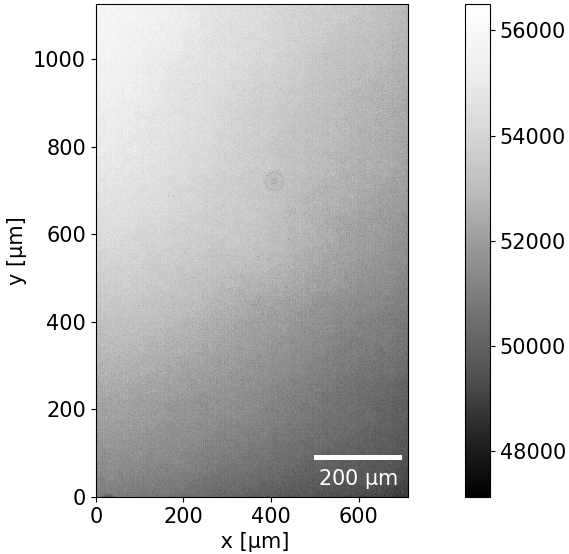
\includegraphics[scale=0.1]{Figs/defectosZEISS/bg_celeste.png}
		\caption{Imagen de fondo de la banda azul del filtro obtenida tomando la mediana para cada píxel de todas las imágenes del barrido.}
		\label{fig:bgazul}
	\end{figure}
	\hspace{0.5cm}En la Figura \ref{fig:bgazul} se muestra la imagen de fondo adquirida para la banda azul, cuya intensidad de la fuente de luz fue configurada en 30$\%$ y el tiempo de integración de la cámara fue de 40 ms. Los dos discos concéntricos que se observan en la imagen son resultado de alguna reflexión no deseada en el microscopio, ya advertida por otros usuarios del equipo. Dichos discos fueron observados en la adquisición de las cinco bandas. Se observa en la imagen de fondo de la Figura \ref{fig:bgazul} que la iluminación del microscopio no es uniforme ya que por ejemplo en la región de la esquina superior izquierda la intensidad de luz es mucho más alta que en la esquina inferior derecha. Por completitud, las imágenes de fondo de cada banda pueden ser descargadas en el siguiente \href{https://drive.google.com/open?id=1LfXvzmIMxf18PmQXzHdFhJl9xa6Ot2BS}{link}.
	
	\item \href{https://github.com/jrr1984/defects_analysis/blob/master/MAIN/bg_normalization.py}{\faGithub} Con la imagen de fondo ya construida, se normalizaron las imágenes originales del barrido completo de una banda\cite{Nordenfelt}. En las Figuras \ref{fig:sinnorm} y \ref{fig:connorm} se muestra una imagen de una \textit{tile} individual del barrido de la banda del NIR antes y después de ser normalizada, respectivamente.	
	
	\begin{figure}[H]
		\begin{floatrow}
			\ffigbox{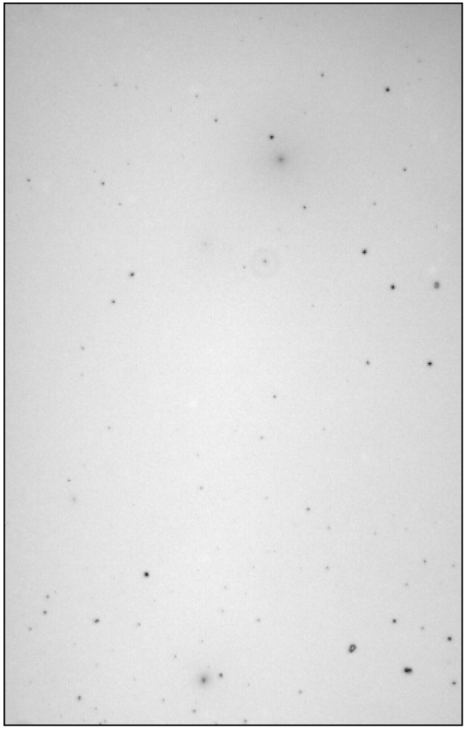
\includegraphics[width=7.0cm,height=10.0cm]{Figs/defectosZEISS/Experiment-11_m001_ORG.png}}{\caption{Imagen original de una \textit{tile} del barrido completo de la banda del NIR. }\label{fig:sinnorm}}
			\ffigbox{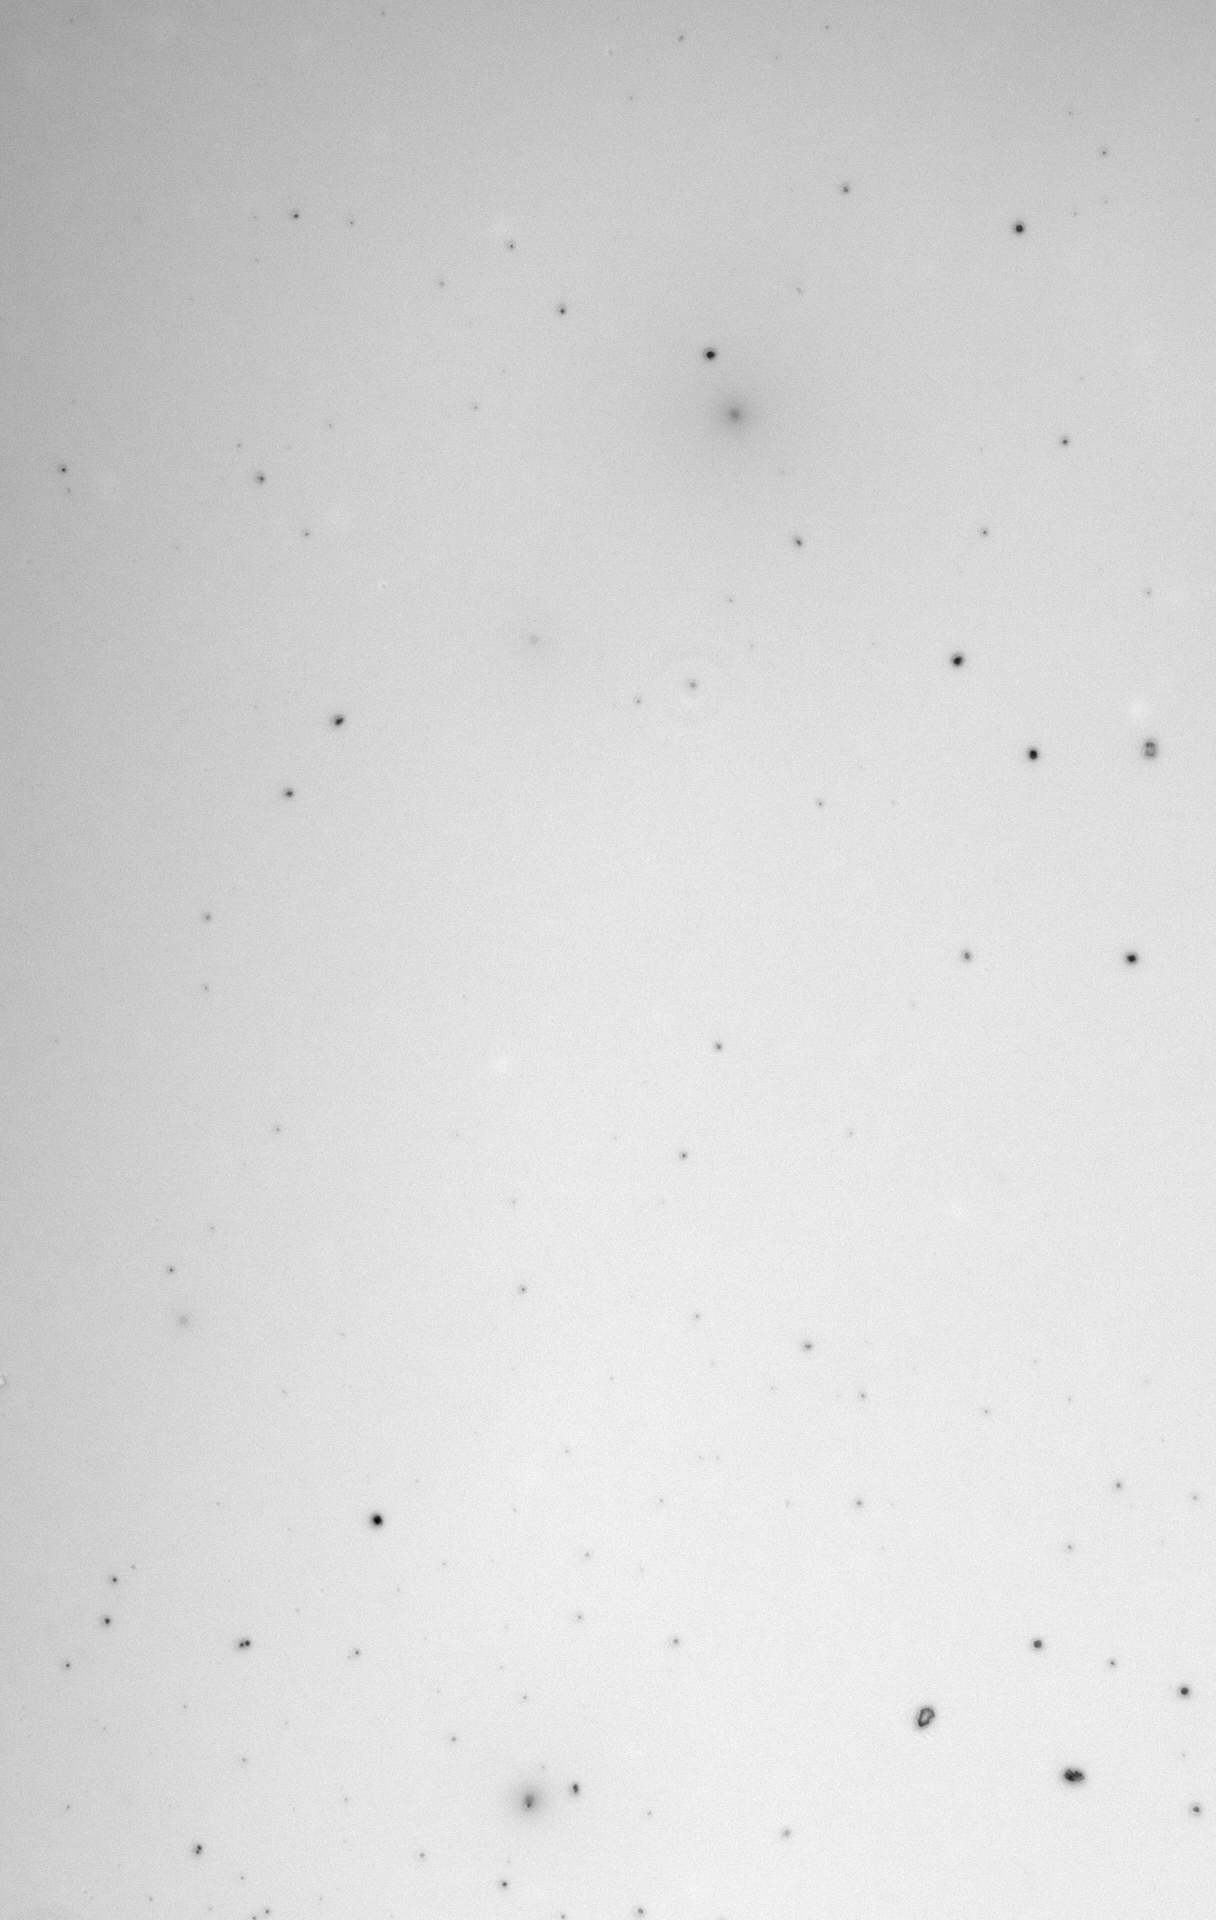
\includegraphics[width=7.0cm,height=10.0cm]{Figs/defectosZEISS/normNIR_1.png}}{\caption{Imagen normalizada a partir de la imagen de fondo.}\label{fig:connorm}}
		\end{floatrow}
	\end{figure}
	
	\vspace{1.0cm}
	\todo[inline]{restar las dos imágenes, mejorar eso.}
	\vspace{1.0cm}
	
\end{enumerate}

\singlespacing
\section{Algoritmo de detección de los defectos}
\spacing{1.5}

\hspace{0.5cm}Con las imágenes pre-procesadas la detección de los defectos fue realizada utilizando algoritmos de procesamientos de imágenes. El algoritmo consistió de los siguientes pasos:
\begin{enumerate}
	\item Se determina el valor de intensidad umbral (en adelante, \textit{threshold}) a partir del cual se distingue entre un defecto en la región de la imagen que se \textit{foreground} y el fondo de la imagen (\textit{background}). %Iterando sobre los conjuntos completos completos de \textit{tiles} de cada banda se determinó que el t
\end{enumerate}





\singlespacing
\section{Resultados del algoritmo de detección de los defectos}
\spacing{1.5}


\hspace{0.5cm}Los resultados del algoritmo de detección de los defectos son guardados en un archivo \textit{pickle}\footnote{Con el módulo \textit{pickle} de python se puede serializar cualquier tipo de objeo de python y guardarse en un archivo \textit{pickle}, de extensión .pkl, que resulta muy eficiente tanto en su escritura como en su lectura.} que puede ser abierto y manipulados sus datos con la librería \textit{pandas} de python en el marco de lo que se conoce como un \textit{pandas dataframe} que no es más que un objeto de python que permite una manipulación de los datos muy eficiente. A continuación se muestra un resumen de los resultados para cada banda espectral del filtro.

\singlespacing
\subsection{Defectos de la banda NIR}
\spacing{1.5}


\begin{figure}[H]
	\centering
	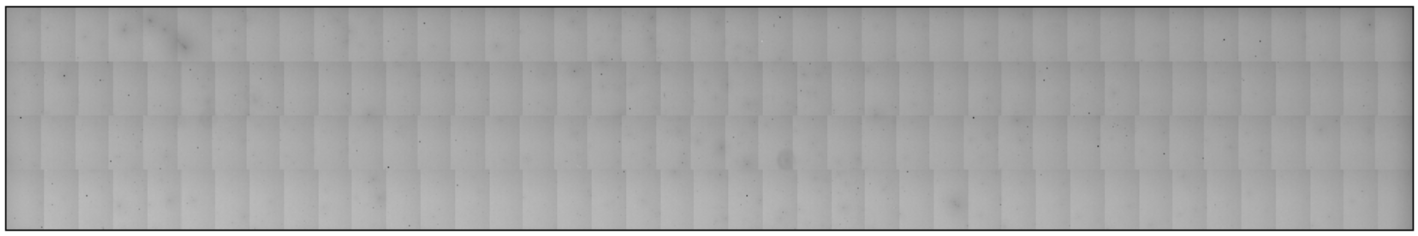
\includegraphics[width=1.0\textwidth,height= 5.0cm]{Figs/resultados_defectos/banda_nir.png}
	\caption{\textit{tile scan} obtenido de la banda NIR de 26.37 mm x 4.16 mm.}
	\label{fig:bgcel}
\end{figure}


\begin{figure}[H]
	\centering
	\includegraphics[width=1.0\textwidth,height= 5.0cm]{Figs/resultados_defectos/tabla_nir.png}
	\caption{Tabla del resumen de resultados del dataframe de la banda NIR.}
	\label{fig:bgcel}
\end{figure}

\singlespacing
\subsection{Defectos de la banda Roja}
\spacing{1.5}


\begin{figure}[H]
	\centering
	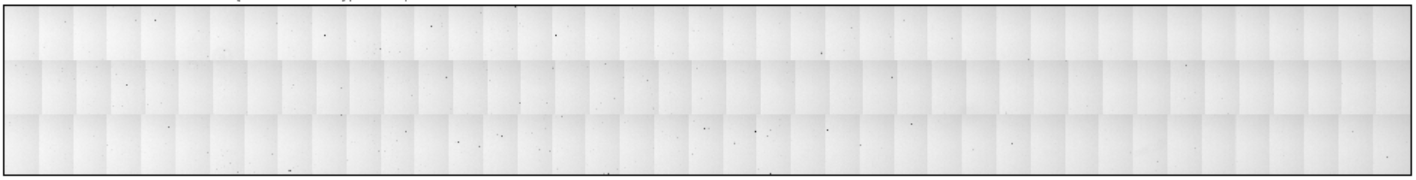
\includegraphics[width=1.0\textwidth,height= 5.0cm]{Figs/resultados_defectos/banda_roja.png}
	\caption{\textit{tile scan} obtenido de la banda roja de 26.37 mm x 3.15 mm.}
	\label{fig:bgcel}
\end{figure}


\begin{figure}[H]
	\centering
	\includegraphics[width=1.0\textwidth,height= 5.0cm]{Figs/resultados_defectos/tabla_roja.png}
	\caption{Tabla del resumen de resultados del dataframe de la banda roja.}
	\label{fig:bgcel}
\end{figure}






El código de este capítulo fue escrito utilizando python 3.6.7 y paquetes numpy 1.17.3, scikit-image 0.16.2 y matplotlib 3.1.2, entre otros.

En el capítulo 3 se realizó una descripción cuantitativa de los defectos: se determinó su tamaño, área, la cantidad de defectos presentes en cada banda. Este tipo de análisis de los defectos sigue la línea de las especificaciones técnicas de \textit{scratch \& dig} y la ISO 10110 en cuanto a que no realizan un análisis cualitativo de los defectos. En el presente trabajo se montó un microespectrómetro para caracterizar espectralmente los defectos. Esto es,

\vspace{1cm}
\todo[inline]{Eventualmente la seccion caracteristicas del filtro va en la introd?}
\vspace{1cm}

 \vspace{1cm}
\todo[inline]{en la seccion caracteristicas del filtro, en el itemize de las bandas..ver de explicar para qué sirve cada banda, usar por ej: \href{http://gspperu.com/pdf/res_landsat7etm.pdf}{link}}
\vspace{1cm}

\vspace{1cm}
\todo[inline]{si hace falta explicar un poco en que consisten los filtros opticos de interferencia..}   
\vspace{1cm}

\vspace{1.0cm}
\todo[inline]{explicar que tipo de lampara es la del Zeiss}
\vspace{1.0cm}

\vspace{1.0cm}
\todo[inline]{Cómo asociar errores a las dimensiones medidas tanto con el fiji como con el algoritmo. Al error de las imágenes del zeiss se le pone la calibración, por ej $\pm$ 0.586 $\mu$m , aprox 0.59 micrones de error }
\vspace{1.0cm}

\vspace{1cm}
\todo[inline]{hace falta explicar las cuentas de la normalizacion de las imagenes.. o que lean la cita de nordenfelt}   
\vspace{1cm}


\vspace{1cm}
\todo[inline]{estimacion de errores, ROI estimacion de falsos positivos falsos negativos tasa de error del sistema, por inspeccion visual nomas}
\vspace{1cm}


\vspace{1cm}
\todo[inline]{ver imagenes y cuantificar cuantos defectos de los mas chicos no agarra, se hace a ojo si o si, revisar banda completa tomando nota de defectos reales vs defectos encontrados y cuantificarlo de alguna manera}
\vspace{1cm}

\vspace{1cm}
\todo[inline]{diagrama de flujo para el algoritmo de deteccion}
\vspace{1cm}

\vspace{1cm}
\todo[inline]{explicar que tipo de lampara es, escuchar audio hernan, poner el codigo de github del espectro con colores facha}
\vspace{1cm}

\vspace{1cm}
\todo[inline]{buscar warning box FACHA}
\vspace{1cm}


\vspace{1cm}
\todo[inline]{Falta: poner siempre la barrita de la escala en las imágenes}
\vspace{1cm}